\documentclass{article}
\usepackage{tikz}
\usetikzlibrary{arrows.meta, positioning}
\usepackage[margin=2cm]{geometry}
\usepackage{amsmath, amssymb}

\tikzset{
  block/.style = {rectangle, draw, text width=7.5em, align=center, rounded corners, minimum height=3em},
  arrow/.style = {draw, -{Latex[length=2mm]}},
}

\begin{document}

\begin{center}
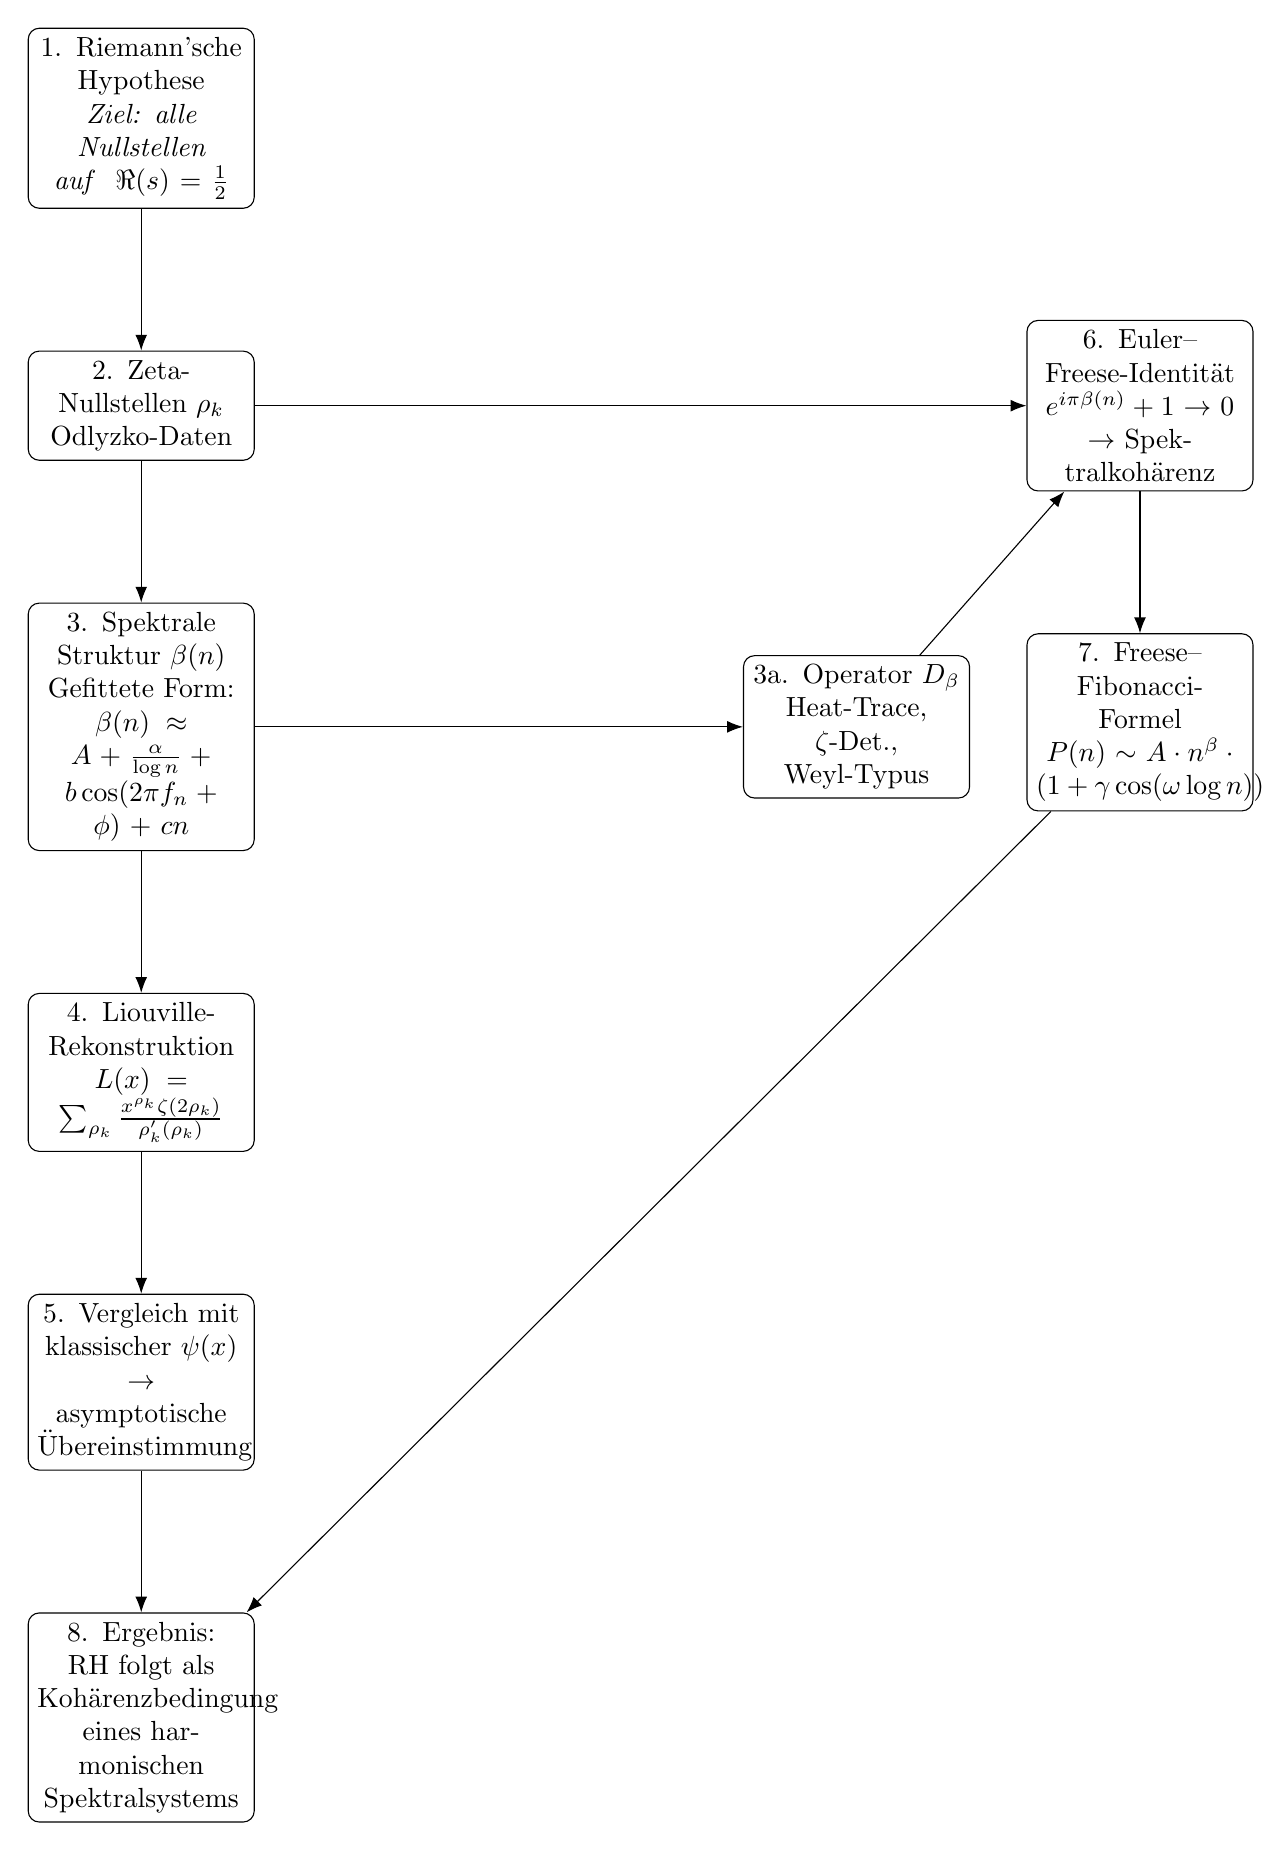
\begin{tikzpicture}[node distance=1.8cm and 2cm]

  \node (1) [block] {1. Riemann'sche Hypothese\\ \textit{Ziel: alle Nullstellen auf } $\Re(s) = \frac{1}{2}$};
  \node (2) [block, below=of 1] {2. Zeta-Nullstellen $\rho_k$\\ Odlyzko-Daten};
  \node (3) [block, below=of 2] {3. Spektrale Struktur $\beta(n)$\\ Gefittete Form:\\ $\beta(n) \approx A + \frac{\alpha}{\log n} + b \cos(2\pi f_n + \phi) + cn$};
  \node (3a) [block, right=of 3, xshift=4.2cm] {3a. Operator $D_\beta$\\ Heat-Trace, $\zeta$-Det.,\\ Weyl-Typus};
  \node (4) [block, below=of 3] {4. Liouville-Rekonstruktion\\ $L(x) = \sum\nolimits_{\rho_k} \frac{x^{\rho_k} \zeta(2\rho_k)}{\rho_k'(\rho_k)}$};
  \node (5) [block, below=of 4] {5. Vergleich mit klassischer $\psi(x)$\\ $\rightarrow$ asymptotische Übereinstimmung};
  \node (6) [block, right=of 2, xshift=7.8cm] {6. Euler--Freese-Identität\\ $e^{i\pi\beta(n)} + 1 \to 0$\\ $\rightarrow$ Spektralkohärenz};
  \node (7) [block, below=of 6] {7. Freese--Fibonacci-Formel\\ $P(n) \sim A \cdot n^\beta \cdot \left(1 + \gamma \cos(\omega \log n) \right)$};
  \node (8) [block, below=of 5] {8. Ergebnis:\\ RH folgt als Kohärenzbedingung eines harmonischen Spektralsystems};

  \draw [arrow] (1) -- (2);
  \draw [arrow] (2) -- (3);
  \draw [arrow] (3) -- (4);
  \draw [arrow] (4) -- (5);
  \draw [arrow] (5) -- (8);
  \draw [arrow] (3) -- (3a);
  \draw [arrow] (3a) -- (6);
  \draw [arrow] (2) -- (6);
  \draw [arrow] (6) -- (7);
  \draw [arrow] (7) -- (8);

\end{tikzpicture}
\end{center}

\end{document}